% !Mode:: "TeX:UTF-8"
\title{实验一 Hadoop集群搭建 实验报告}
\author{江昱峰 21009200038} 
\documentclass {article}
\usepackage[UTF8]{ctex}
\usepackage{graphicx}
\usepackage{float}
\usepackage{hyperref}
\usepackage{makecell}
\begin{document}
	%\begin{sloppypar}
	\maketitle{}
	\section{背景介绍}
		Hadoop是一个开源的分布式计算框架,用于处理大规模数据集的存储和处理。它提供了可靠性、可扩展性和容错性,使得用户能够在集群中并行处理大量数据。Hadoop的核心组件包括Hadoop分布式文件系统(HDFS)和MapReduce计算模型。
		
		在大数据时代,数据量的不断增长对传统的数据处理和存储方式提出了挑战。传统的单机系统无法满足处理大规模数据集的需求,因此需要分布式计算框架来解决这个问题。Hadoop应运而生,成为处理大数据的重要工具。
		
	\section{实验目的}
		实践并掌握Hadoop集群搭建,具体包括以下四部分内容:
		\begin{itemize}
			\item Linux环境配置;
			\item HDFS伪分布式集群搭建;
			\item YARN伪分布式集群搭建;
			\item 基于Hadoop的PI值计算。
		\end{itemize}
	
	\section{环境配置目的}
		\begin{itemize}
			\item Hadoop是Java程序进程,在学习Hadoop体系时,必须要有JDK环境作为支撑。
			\item JDK(Java Development Kit)即Java开发工具,安装需要配置环境变量(JAVA\_HOME,PATH),目的是用到JDK程序和编译命令文件时方便在任意目录下可以找到。
			\item SSH(Secure Shell)是一个建立在应用层上的安全远程管理,可靠地传输协议。为远程连接提供安全,防止远程管理信息泄露。
			\item 在实际环境当中,服务器部署在机房,为方便开发人员操作,可通过远程连接控制操作。
			\item 集群中主节点访问需要不断获取从节点服务用户密码,通过配置SSH远程免密登录,解决之间频繁获取用户密码问题。
		\end{itemize}
	
	\section{实验知识}	
		\begin{itemize}
			\item JDK介绍:JDK是Java Development Kit的缩写,中文称为Java开发工具包,由SUN公司提供。它为Java程序开发提供了编译和运行环境,所有的Java程序的编写都依赖于它。使用JDK可以将Java程序编写为字节码文件,即 .class文件。
			\item SSH免密介绍:SSH为Secure Shell(安全外壳协议) 的缩写。SSH是一种网络协议,用于计算机之间的加密登录。很多ftp、pop和telnet在本质上都是不安全的,因为它们在网络上用明文传送口令和数据,别有用心的人非常容易就可以截获这些口令和数据。SSH就是专为远程登录会话和其他网络服务提供安全性的协议。
			\item Hadoop介绍:Hadoop是一个由Apache基金会所开发的分布式系统基础架构。用户可以在不了解分布式底层细节的情况下,开发分布式程序。充分利用集群的威力进行高速运算和存储。允许使用简单的编程模型在大量计算机集群上对大型数据集进行分布式处理。
			\item YARN集群概述:Yarn是随着Hadoop发展而催生的新框架,全称是Yet Another Resource Negotiator,可以翻译为“另一个资源管理器”。Yarn取代了以前Hadoop中JobTracker的角色,因为以前JT的任务过重,负责任务的调度、跟踪、失败重启等过程,而且只能运行MapReduce作业,不支持其他编程模式,这也限制了JT使用范围,而Yarn应运而生,解决了这两个问题。用户可以将各种服务框架部署在YARN上,由YARN进行统一地管理和资源分配。
		\end{itemize}
	
	\section{实验要求}
		完成Hadoop集群搭建,具体包括以下四部分任务:
		\begin{itemize}
			\item Linux环境配置;
			\item HDFS伪分布式集群搭建;
			\item YARN伪分布式集群搭建;
			\item 基于Hadoop的PI值计算。
		\end{itemize}
	
	\section{实验原理}
		PI值计算原理:
		\begin{figure}[H]
			\centering
			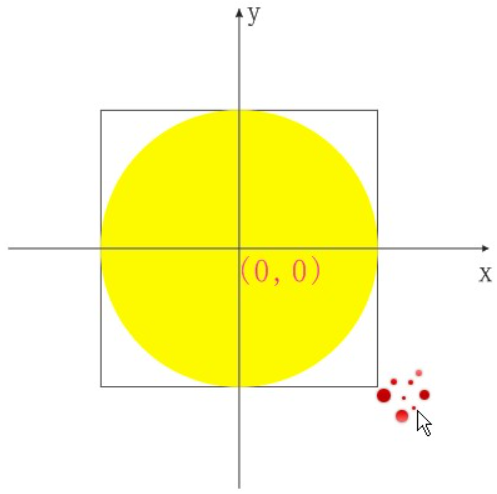
\includegraphics[width=4in,height=4in]{figures/fig1.jpg}
		\end{figure}

		假如有一个边长为2的正方形。以正方形的一个中心点为圆心,以1为半径,画一个圆,于是在正方形内就有了一个内切圆。在正方形里随机生成若干个点,则有些点是在圆内,有些点是在圆外。正方形的面积是4,圆的面积是Pi。设点的数量一共是Max\_DAST,圆内的点数量是PI\_DAST,在点足够多足够密集的情况下,会近似有PI\_DAST/Max\_DAST的比值约等于圆面积与正方形面积的比值,也就是PI\_DAST/Max\_DAST= Pi/2*2,即$Pi=4*PI\_DAST/Max\_DAST$。
	
	\section{实验环境}
		本次实验实验环境为青椒课堂平台的Linux(Centos 7.5)操作系统。
	
	\section{实验步骤与结果截图}
		\subsection{Linux环境配置}
			\subsubsection{任务1:解压缩JDK安装包}
				环境当中已经将安装包提供,可直接使用。JDK安装包所在路径:/root/software/jdk-8u221-linux-x64.tar.gz。
				
				解压缩步骤:
				\begin{enumerate}
					\item 进入/root/software/目录下。
						\begin{figure}[H]
							\centering
							
\includegraphics{figures/fig2.jpg}
						\end{figure}
					
					\item 解压安装包到当前目录。
						\begin{figure}[H]
							\centering
							
\includegraphics[width=4.5in]{figures/fig3.jpg}
						\end{figure}
					
					\item 查看/root/software/目录下解压文件。
						\begin{figure}[H]
							\centering
							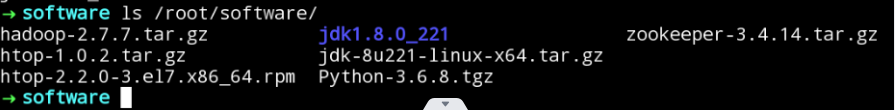
\includegraphics[width=4.5in]{figures/fig4.jpg}
						\end{figure}
				\end{enumerate}
		
			\subsubsection{任务2:配置JDK环境变量}
				配置环境变量步骤:
				\begin{enumerate}
					\item 编辑系统环境变量文件 /etc/profile。
						\begin{figure}[H]
							\centering
							
\includegraphics{figures/fig5.png}
						\end{figure}
					
					\item 在末尾添加JDK的安装目录以及PATH路径添加JDK安装路径。
						\begin{figure}[H]
							\centering
							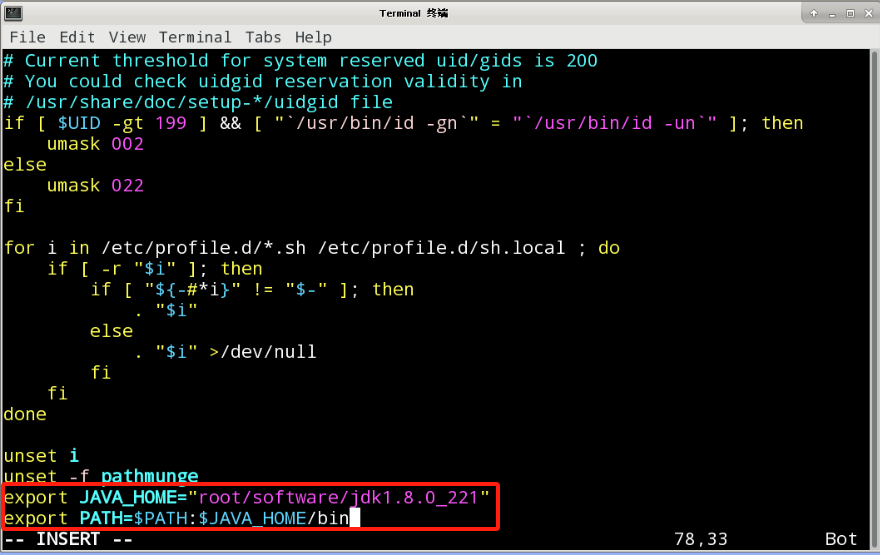
\includegraphics[width=4.5in]{figures/fig6.png}
						\end{figure}
					
					\item 使用source 命令使配置文件生效。
						\begin{figure}[H]
							\centering
							
\includegraphics[width=4.5in]{figures/fig7.jpg}
						\end{figure}
					
					\item 通过检测命令检测JDK环境安装是否成功。
						\begin{figure}[H]
							\centering
							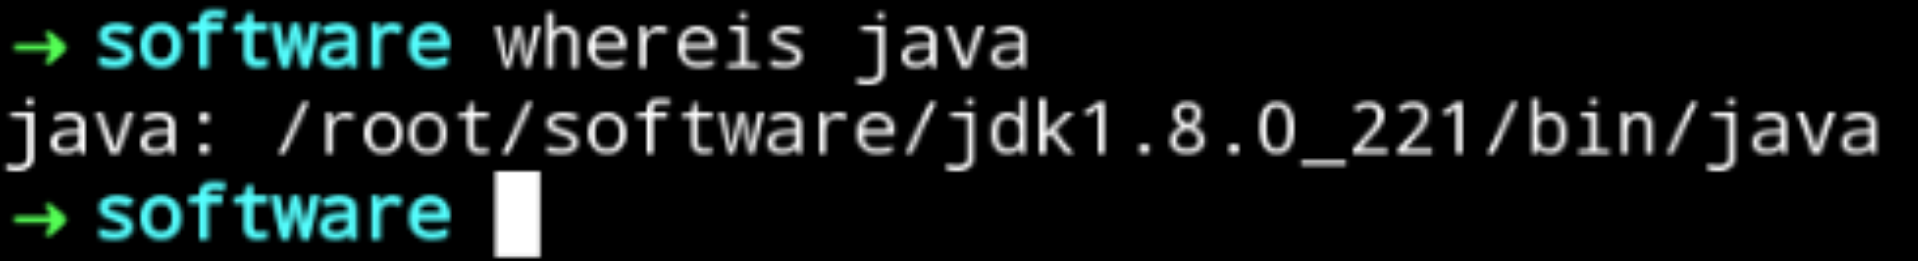
\includegraphics[width=4.5in]{figures/fig8.jpg}
						\end{figure}
				\end{enumerate}
			
			\subsubsection{任务3:SSH服务获取公钥私钥}
				环境当中已经下载好SSH服务(openssh-server和openssh-clients),直接进行操作即可。有两种免密方式,选择两者中任意一种方式即可。此处我选择非对称算法RSA。
							
				SSH免密流程:
				\begin{enumerate}
					\item 启动SSH服务。
						\begin{figure}[H]
							\centering
							
\includegraphics{figures/fig9.jpg}
						\end{figure}
					
					\item 使用netstat命令查看端口号。
						\begin{figure}[H]
							\centering
							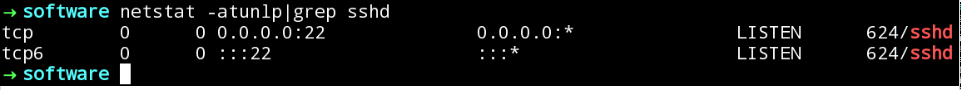
\includegraphics[width=4.5in]{figures/fig10.jpg}
						\end{figure}
					
					\item 使用RSA算法生成密钥对。输入信息时不需要输入,回车三次即可。
						\begin{figure}[H]
							\centering
							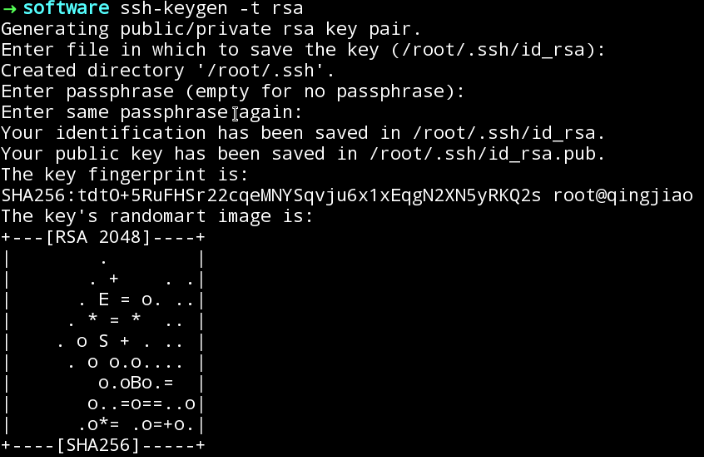
\includegraphics[width=4.5in]{figures/fig11.jpg}
						\end{figure}
					
					\item 查看/root/.ssh 路径下生成的公钥私钥文件。
						\begin{figure}[H]
							\centering
							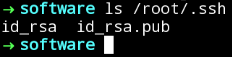
\includegraphics{figures/fig12.png}
						\end{figure}
				\end{enumerate}
		
			\subsubsection{任务4:SSH授权并验证登录}
				本节任务对SSH免密进行授权,使用方式与上一任务使用方式保持一致,否则授权失败。
				\begin{enumerate}
					\item 将获取的公钥文件id\_rsa.pub拷贝到授权列表文件authorized\_keys 。
						\begin{figure}[H]
							\centering
							
\includegraphics{figures/fig13.jpg}
						\end{figure}
					
					\item 修改授权列表文件 authorized\_keys的权限,使拥有者可读可写,其他用户无权限。
						\begin{figure}[H]
							\centering
							
\includegraphics{figures/fig14.jpg}
						\end{figure}
					
					\item 通过hostname 命令获取本机名。
						\begin{figure}[H]
							\centering
							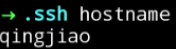
\includegraphics{figures/fig15.jpg}
						\end{figure}
					
					\item 验证免密登录是否配置成功(查看/root目录方式验证)。确保提交检测完成之后才可进行退出操作。
						\begin{figure}[H]
							\centering
							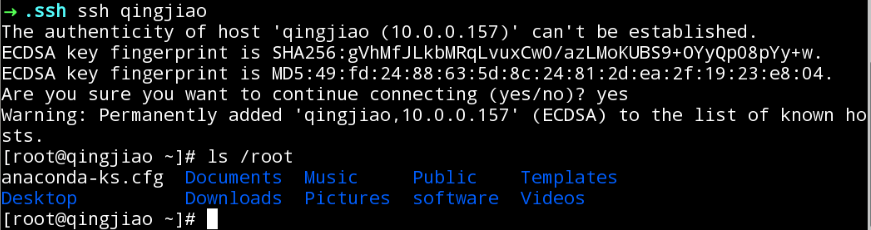
\includegraphics[width=4.5in]{figures/fig16.jpg} 
						\end{figure}
				\end{enumerate}

		\subsection{HDFS伪分布式集群搭建}
			\subsubsection{任务1:检测JDK环境,解压安装包}
				\begin{enumerate}
					\item 使用java -version命令检测JDK环境是否安装成功(安装Hadoop集群必须有JAVA环境)。
						\begin{figure}[H]
							\centering
							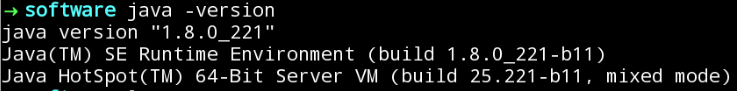
\includegraphics[width=4.5in]{figures/fig17.png}
						\end{figure}
					
					\item 解压Hadoop安装包,安装包已下载,存放在 /root/software/ 目录下,进入到目录,解压安装包到当前文件。
						\begin{figure}[H]
							\centering
							
\includegraphics{figures/fig18.png}
						\end{figure}
					
					\item 查看当前目录结构,查看解压是否成功。
						\begin{figure}[H]
							\centering
							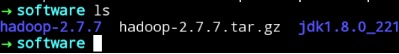
\includegraphics{figures/fig19.jpg}
						\end{figure}
				\end{enumerate}
		
			\subsubsection{任务2:配置文件}
				\begin{enumerate}
					\item 编辑hadoop-env.sh,修改JAVA\_HOME参数为本机JDK所在路径(/root/software/jdk1.8.0\_221)。
					\begin{figure}[H]
						\centering
						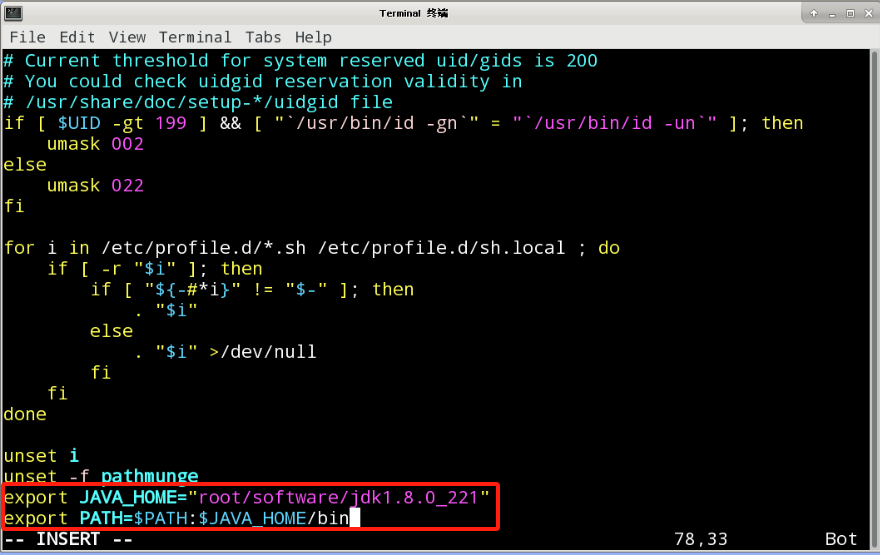
\includegraphics[width=4.5in]{figures/fig20.png}
					\end{figure}
				
					\item 配置核心组件core-site.xml,在配置<configuration></configuration>中添加如下内容:
					\begin{figure}[H]
						\centering
						
\includegraphics{figures/fig21.png}
					\end{figure}
				
					\begin{figure}[H]
						\centering
						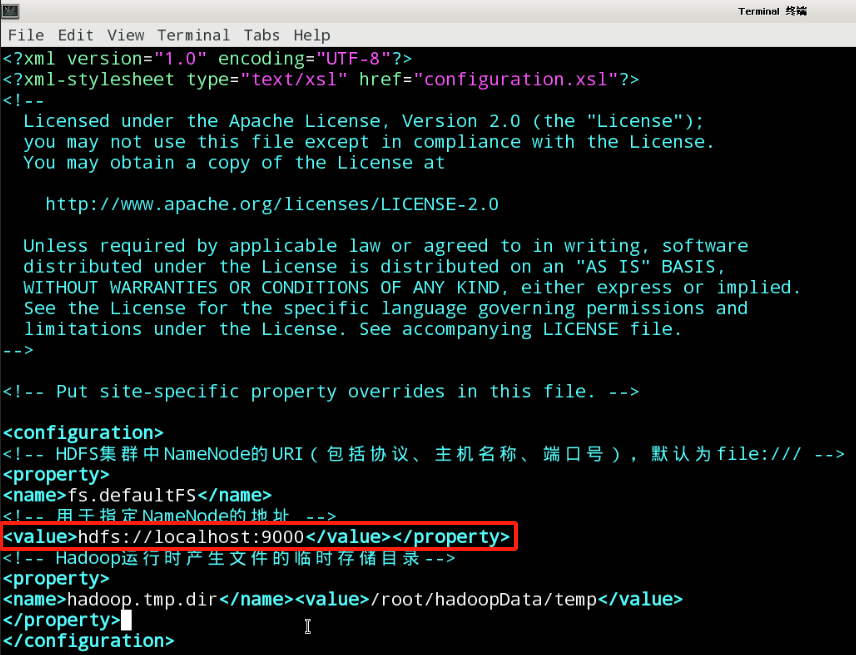
\includegraphics[width=4.5in]{figures/fig22.png}
					\end{figure}
				
					\item 配置文件系统hdfs-site.xml,添加如下内容:
					\begin{figure}[H]
						\centering
						
\includegraphics{figures/fig23.png}
					\end{figure}
					\begin{figure}[H]
						\centering
						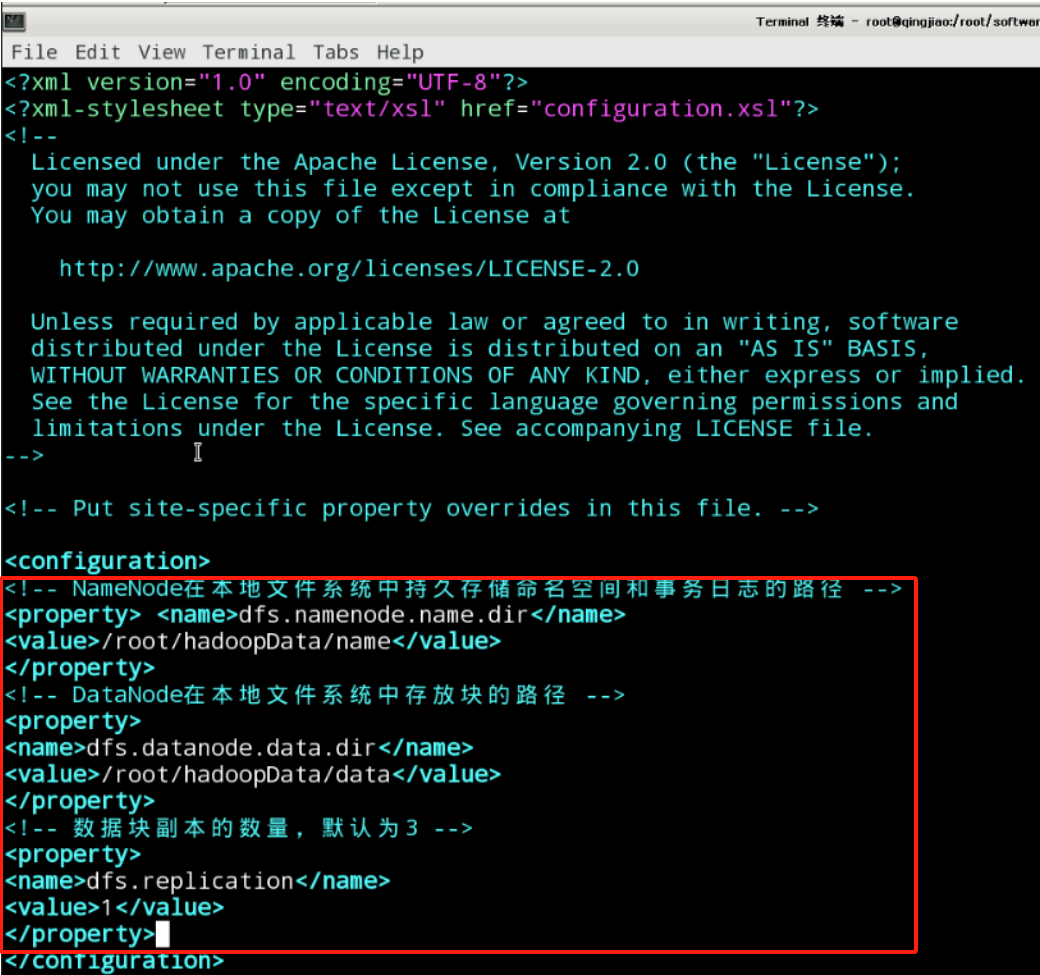
\includegraphics[width=4.5in]{figures/fig24.jpg}
					\end{figure}
				
					\item 配置slaves文件,修改从节点主机名为本主机名。(见上图)
				\end{enumerate}
		
			\subsubsection{任务3:配置Hadoop环境变量}
				\begin{enumerate}
					\item 打开/etc/profile 文件,添加HADOOP\_HOME 路径和PATH路径。
					\begin{figure}[H]
						\centering
						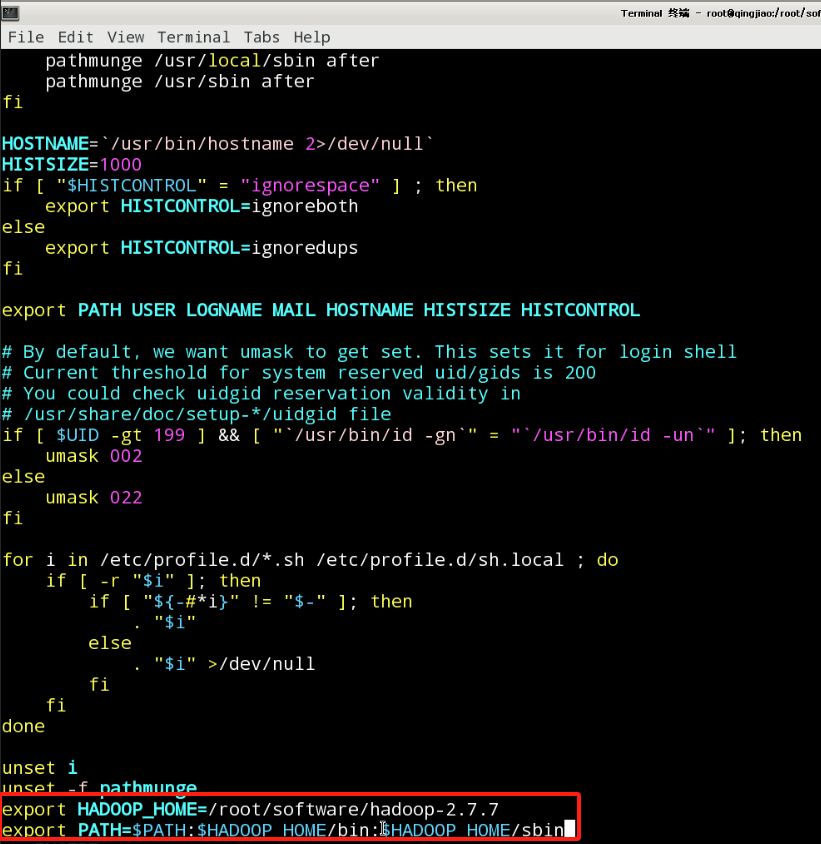
\includegraphics[width=4.5in]{figures/fig25.png}
					\end{figure}
				
					\item 使用source配置文件立即生效。
					\begin{figure}[H]
						\centering
						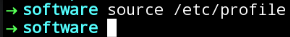
\includegraphics{figures/fig26.png}
					\end{figure}
				
					\item 使用命令检测Hadoop环境变量是否设置成功。
					\begin{figure}[H]
						\centering
						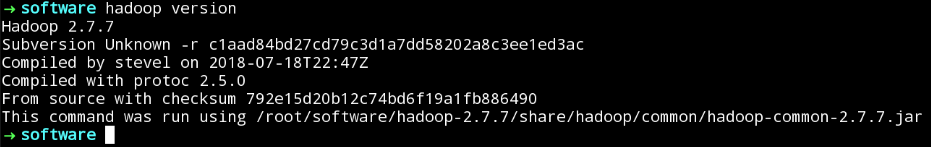
\includegraphics[width=4.5in]{figures/fig27.png}
					\end{figure}
				\end{enumerate}
				
			\subsubsection{任务4:HDFS集群测试}
				\begin{enumerate}
					\item 格式化文件系统。(格式化文件系统仅用于第一次启动HDFS)
					\begin{figure}[H]
						\centering
						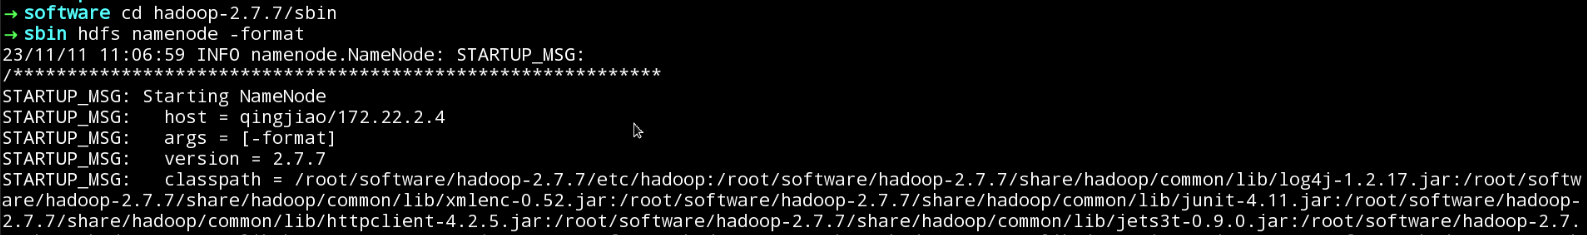
\includegraphics[width=4.5in]{figures/fig28.png}
					\end{figure}
				
					\item 使用脚本命令一键启动。
					\begin{figure}[H]
						\centering
						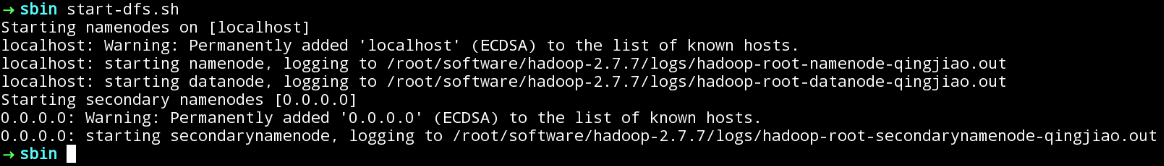
\includegraphics[width=4.5in]{figures/fig29.png}
					\end{figure}
				
					\item 查看进程启动情况。
					\begin{figure}[H]
						\centering
						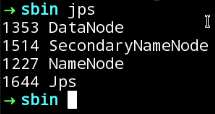
\includegraphics{figures/fig30.png}
					\end{figure}
				
					\item 使用脚本命令一键退出。
					\begin{figure}[H]
						\centering
						
\includegraphics{figures/fig31.png}
					\end{figure}
				\end{enumerate}
			
		\subsection{YARN伪分布式集群搭建}
			\subsubsection{任务1:配置环境变量}
				配置环境变量yarn-env.sh:
				\begin{enumerate}
					\item 使用命令查看是否存在jdk环境,通过echo命令获取本机JDK所在路径。
					\begin{figure}[H]
						\centering
						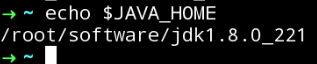
\includegraphics{figures/fig32.png}
					\end{figure}
				
					\item 使用命令打开yarn-env.sh文件。
					\begin{figure}[H]
						\centering
						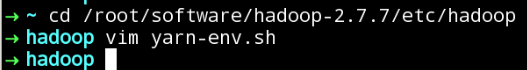
\includegraphics{figures/fig33.png}
					\end{figure}
				
					\item 修改JAVA\_HOME参数为本机JDK所在路径。
					\begin{figure}[H]
						\centering
						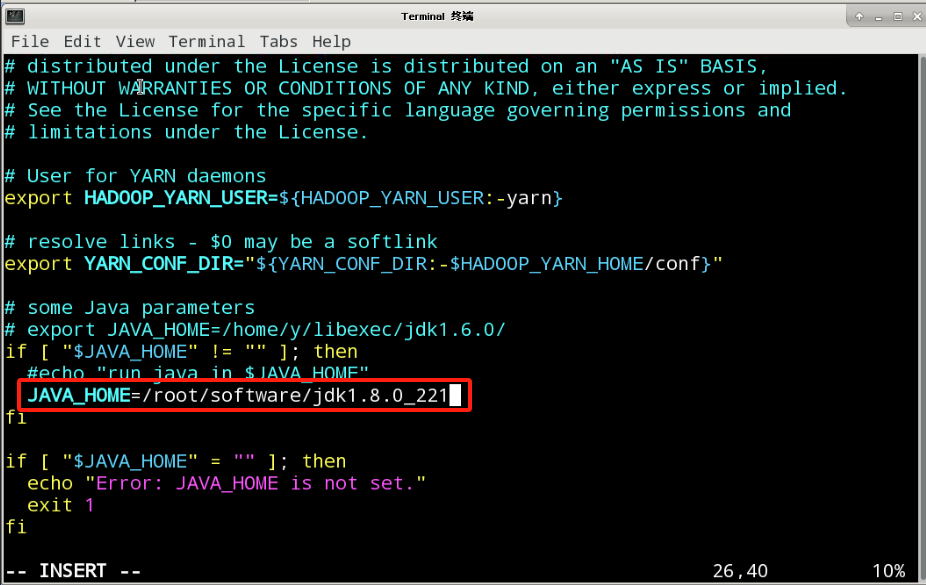
\includegraphics[width=4.5in]{figures/fig34.png}
					\end{figure}
				\end{enumerate}
			
			\subsubsection{任务2:配置计算框架}
				配置计算框架mapred-site.xml
				\begin{enumerate}
					\item 进入\$HADOOP\_HOME/etc/hadoop/目录下将mapred-site.xml.template文件复制并改名为mapred-site.xml。
					\begin{figure}[H]
						\centering
						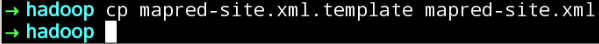
\includegraphics[width=4.5in]{figures/fig35.png}
					\end{figure}
				
					\item 打开mapred-site.xml文件,进入编辑模式。
					\begin{figure}[H]
						\centering
						
\includegraphics{figures/fig36.png}
					\end{figure}
				
					\item 添加内容。
					\begin{figure}[H]
						\centering
						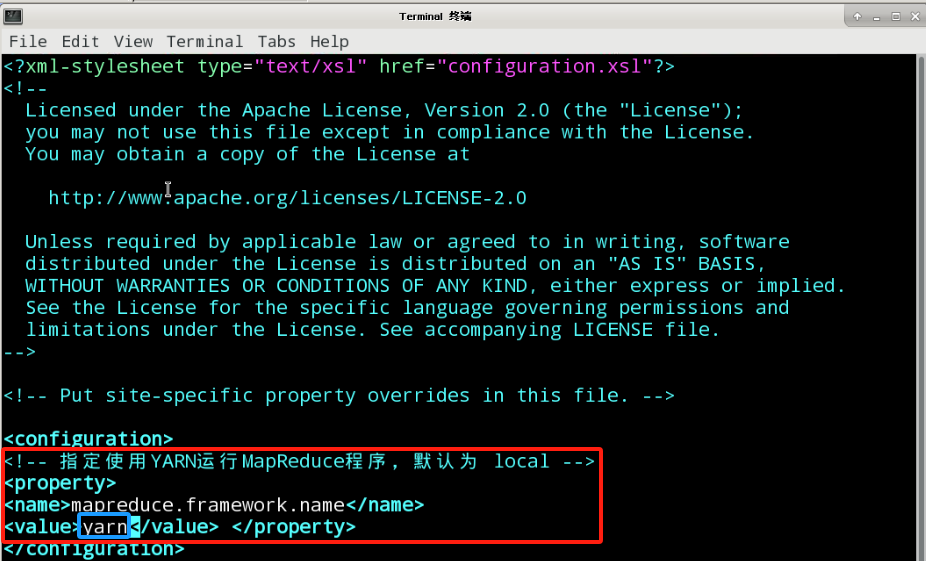
\includegraphics[width=4.5in]{figures/fig37.png}
					\end{figure}
				\end{enumerate}
			
			\subsubsection{任务3:配置YARN系统}
				配置YARN系统yarn-site.xml。
				\begin{enumerate}
					\item 打开YARN核心配置文件yarn-site.xml。
					\begin{figure}[H]
						\centering
						
\includegraphics{figures/fig38.png}
					\end{figure}
				
					\item 在文件<configuration></configuration>中间添加配置内容:
					\begin{figure}[H]
						\centering
						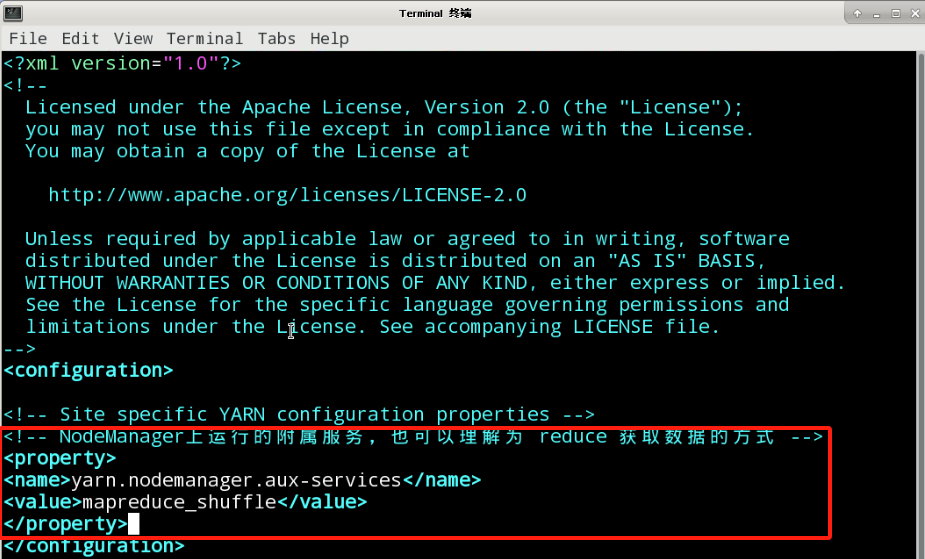
\includegraphics[width=4.5in]{figures/fig39.png}
					\end{figure}
				\end{enumerate}		
					
			\subsubsection{任务4:启动检测YARN集群}
				YARN伪分布式集群检测:
				\begin{enumerate}
					\item 使用脚本命令一键启动YARN集群。
					\begin{figure}[H]
						\centering
						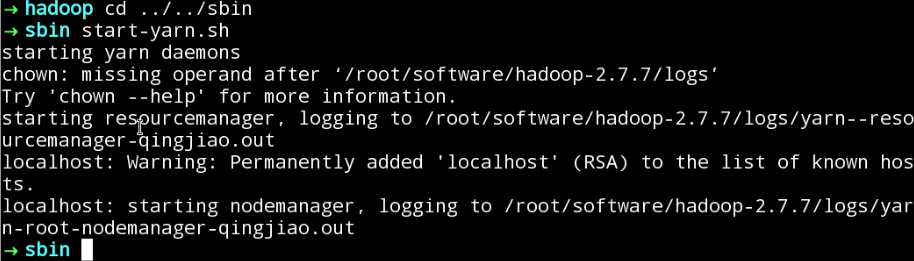
\includegraphics[width=4.5in]{figures/fig40.png}
					\end{figure}
				
					\item 查看进程是否启动ResourceManager和NodeManager。
					\begin{figure}[H]
						\centering
						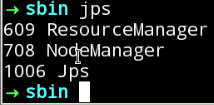
\includegraphics{figures/fig41.png}
					\end{figure}
				
					\item 使用脚本命令一键关闭YARN集群。
					\begin{figure}[H]
						\centering
						
\includegraphics{figures/fig42.png}
					\end{figure}
				\end{enumerate}
		
		\subsection{Hadoop初体验——PI值计算}
			任务1:PI值计算实现步骤:
			\begin{enumerate}
				\item 启动Hadoop集群,系统环境已经启动。可通过jps命令进行查看。
				\begin{figure}[H]
					\centering
					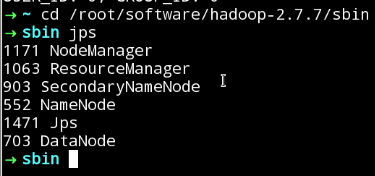
\includegraphics{figures/fig43.png}
				\end{figure}
			
				\item 进入到官方提供jar包目录\$HADOOP\_HOME/share/hadoop/mapreduce/。
				\begin{figure}[H]
					\centering
					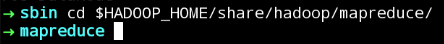
\includegraphics{figures/fig44.png}
				\end{figure}
			
				\item 通过查看命令查看目录下PI值计算所用jar包。
				\item 使用命令运行该jar包并指定map数为10,总点数为100。
				\begin{figure}[H]
					\centering
					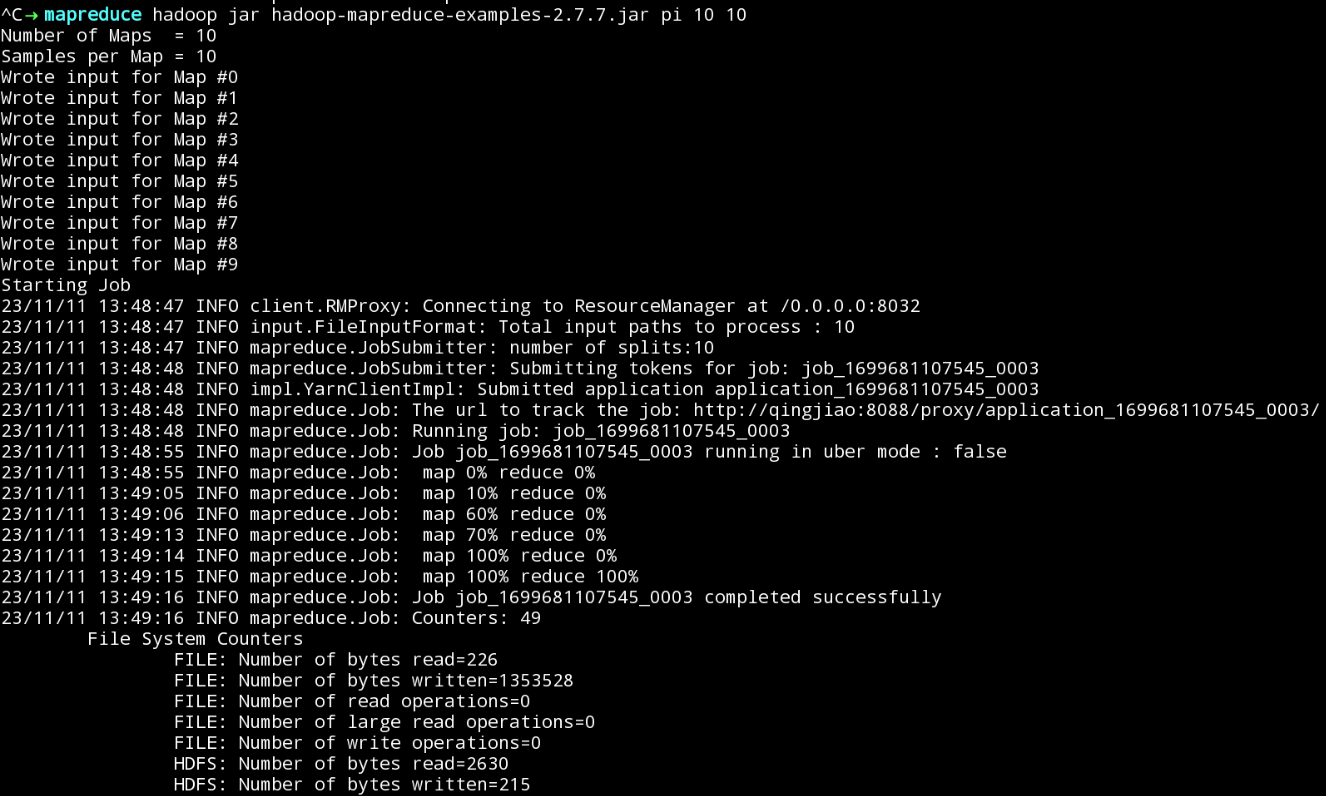
\includegraphics[width=4.5in]{figures/fig45.png}
				\end{figure}
			
				\item 查看计算结果并进行记录。
				\begin{figure}[H]
					\centering
					
\includegraphics{figures/fig46.png}
				\end{figure}
				
				计算结果为3.2000。
				\item 使用命令再次运行该jar包并指定map数为100,总点数为10000。
				\begin{figure}[H]
					\centering
					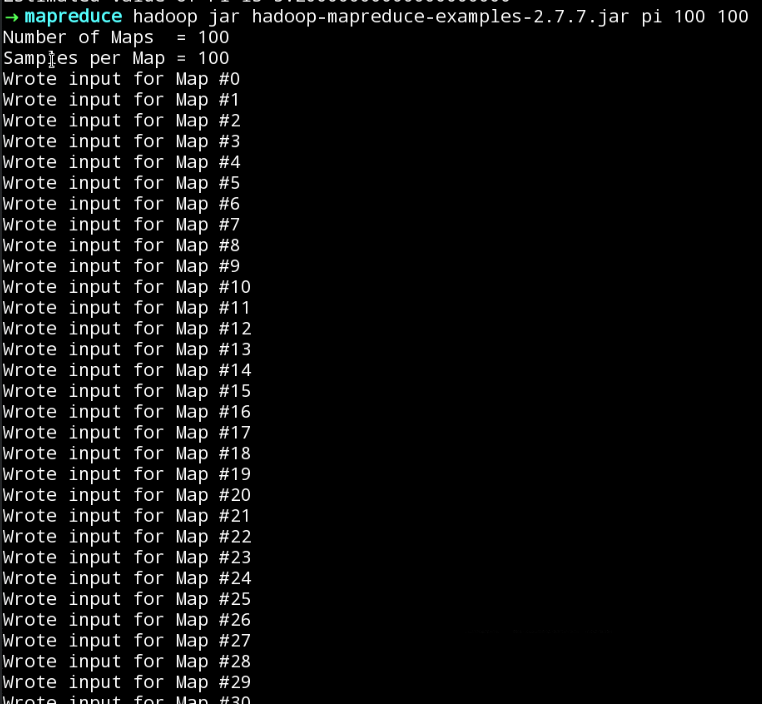
\includegraphics[width=4.5in]{figures/fig47.png}
				\end{figure}
			
				\item 再次查看计算结果并和上次计算结果对比。
				\begin{figure}[H]
					\centering
					
\includegraphics{figures/fig48.png}
				\end{figure}
			
				计算结果为3.1408。
			\end{enumerate}

	\section{结果分析}
		就总体趋势而言,当mapreduce的切片越细,即map、总点数越大时,计算结果越精确。
	
	\section{困难解决}
		1.1.4(任务4:SSH授权并验证登录)部分在原账号对应平台上用"ssh qingjiao "ls /root""命令虽然能成功执行但无法通过检测,后将此命令拆成"ssh qingjiao"和"ls /root"两个命令分别执行,成功通过检测。
	
	\section{心得体会}
		做完本次实验,除了掌握了实验目的部分中所有内容的收获之外,我还有以下几点心得体会:
		\begin{itemize}
			\item 实践并掌握了SSH服务获取公钥私钥、SSH授权并验证登录、配置Hadoop环境变量、配置计算框架、配置YARN系统等内容。
			\item 对比分析了HDFS伪分布式集群搭建、YARN伪分布式集群搭建的异同点。
			\item 基于Hadoop进行了编程实操。
		\end{itemize}
%\end{sloppypar}
\end{document}
\endinput